% main.tex - paper 2 (JINST): hit-level background rejection in the inner and outer trackers of a
% muon collider (barrel, intermediate and endcap regions) and the resolutions it requires, using
% the fake-track lower limit of paper 1.
% Draft 3, 14 October 2026. Numbers: run 2026-10-14_162239_pdf (100 um, 100 ps, 1.5 deg) and
% the resolution scans around it (claude_scratch/op100); figures from make_figures.py.
%
% Build:  pdflatex main && bibtex main && pdflatex main && pdflatex main
\IfFileExists{jinst.cls}{\documentclass[a4paper,11pt]{jinst}}
  {\documentclass[a4paper,11pt]{article}\usepackage{jinst-fallback}}
\usepackage{amsmath,amssymb,graphicx,xcolor,booktabs}

\newcommand{\ndof}{n_\mathrm{dof}}
\newcommand{\pT}{p_T}
\newcommand{\tc}{t_\mathrm{corr}}
\newcommand{\todo}[1]{\textcolor{red!70!black}{[#1]}}

\title{Beam-induced background rejection with hit timing and direction in the tracker of a muon
collider, and the resolutions it requires}

\author[a]{M.~Casarsa}
\author[b,1]{L.~Ristori\note{Corresponding author.}}
\affiliation[a]{INFN, Sezione di Trieste, Trieste, Italy}
\affiliation[b]{Fermi National Accelerator Laboratory, Batavia, IL 60510, USA}
\emailAdd{luciano@fnal.gov}

\abstract{At a 10~TeV muon collider the decays of the circulating muons fill the tracker with
millions of background hits per bunch crossing. We study how far this beam-induced background
can be reduced hit by hit, before any pattern recognition, if every hit carries a time and a
direction measurement, and what that implies for track reconstruction in the inner and outer
trackers. Three cuts test whether a hit is compatible with a particle coming
from the interaction point: on its time corrected for the time of flight, on the extrapolation
of its direction to the beam axis, and on the transverse momentum implied by its direction.
With a position resolution of 100~$\mu$m, a time resolution of 100~ps and a direction
resolution of $1.5^\circ$, and cuts set to keep 98\% of the signal hits each, the background
in the inner and outer trackers is reduced by a factor of 57 while 97\% of the hits of signal
muons and 98\% of the tracks are kept. The algorithm-independent lower limit on combinatorial
fake tracks of a companion paper then gives $1.9\times10^{-2}$ fakes per bunch crossing: $1.7\times10^{-2}$
in the barrel, $1.7\times10^{-3}$ in the region where tracks cross both barrel layers and endcap
disks, and $1.5\times10^{-6}$ in the endcaps. One fake per crossing would be reached at 2.2 times the
simulated background density. Scans
of the three resolutions show how this margin depends on each of them and set targets for
detector R\&D.}

\keywords{Pattern recognition, cluster finding, calibration and fitting methods; Performance of
High Energy Physics Detectors; Timing detectors; Particle tracking detectors}

\begin{document}
\flushbottom
\maketitle

% =====================================================================
\section{Introduction}\label{sec:intro}

A multi-TeV muon collider would combine the discovery reach of a hadron collider of much
higher energy with the clean final states of lepton
collisions~\cite{Accettura:2023,IMCC:2024interim}. The price, for the detector, is the
beam-induced background (BIB): the decay products of the circulating muons interact with the
machine elements near the interaction region and reach the detector as a diffuse flux of
low-energy photons, electrons, neutrons and charged hadrons, out of time and out of direction
with respect to the collisions~\cite{Bartosik:2020,Collamati:2021,Casarsa:2024review}. In the
tracker this flux produces millions of hits per bunch crossing, with densities above one hit per
mm$^2$ in the innermost layers, and the reconstruction of charged tracks among them is the
central challenge of the tracker design.

Several handles against the BIB are known. The hits arrive spread over a few nanoseconds while
those of particles from the collision arrive within tens of picoseconds of the expected time of
flight, so a timing window removes much of the
background~\cite{Bartosik:2020,Casarsa:2024review}. The BIB particles also cross the sensors at
directions unrelated to the interaction point, which double-layer sensors or cluster shapes can
exploit. Full reconstruction chains built on these ideas, and the detector concepts proposed for a
10~TeV collider~\cite{Andreetto:2026music,Bell:2025maia}, show that tracking is possible, with
rates of fake tracks that depend on the algorithm used.

This paper asks a complementary question. If every hit carries a time and a direction, how much of
the BIB can be removed hit by hit, before any pattern recognition, while keeping nearly all the hits
of particles from the interaction point; and does what remains still allow tracks to be found by
\emph{any} algorithm? The first part is a selection on three per-hit observables, each testing the
compatibility of the hit with a particle produced at the interaction point. The second uses the
algorithm-independent lower limit on combinatorial fake tracks derived in a companion
paper~\cite{Paper1}: the expected number of combinations of background hits that pass the same
goodness-of-fit cut as real tracks, which no algorithm keeping the efficiency for real tracks can
reject. Both are evaluated for the inner and outer trackers, where the limit is computed from the
measured hit densities, layer by layer, in three regions: the barrel, the endcaps, and the
intermediate region in which tracks cross both barrel layers and endcap disks. Finally, scanning the
position, time and direction resolutions shows how much margin the selection leaves and which
resolution matters most. The direction measurement in particular is treated as a capability to be
developed: the scans give the precision it would need.

Section~\ref{sec:samples} describes the simulated samples and the detector, section~\ref{sec:obs}
the per-hit observables and section~\ref{sec:selection} the selection and its performance.
Section~\ref{sec:fakes} applies the fake-track limit to the three regions, section~\ref{sec:scans}
presents the resolution scans and section~\ref{sec:discussion} discusses the limitations.

% =====================================================================
\section{Simulated samples and detector}\label{sec:samples}

\paragraph{Detector.} We use the MUSIC detector concept for a 10~TeV muon
collider~\cite{Andreetto:2026music} \todo{confirm the geometry version and the reference}, with a
5~T solenoidal field. Its tracker consists of a vertex detector (VXD), an inner tracker (IT) and
an outer tracker (OT), each with a barrel and two endcaps. This paper concerns the IT and OT. Their
barrels have three IT layers at radii of 165, 355 and 555~mm and three OT layers at 820, 1154 and
1491~mm; each endcap has seven IT disks between $|z|=606$ and 2192~mm and four OT disks between
1408 and 2192~mm (table~\ref{tab:layers}). The vertex detector is not used: its hits do not count
towards the track-finding criterion and its layers are not included in the fake-track limit. The
sensitive areas are taken from the geometry description of the modules.

\begin{figure}[htbp]
  \centering
  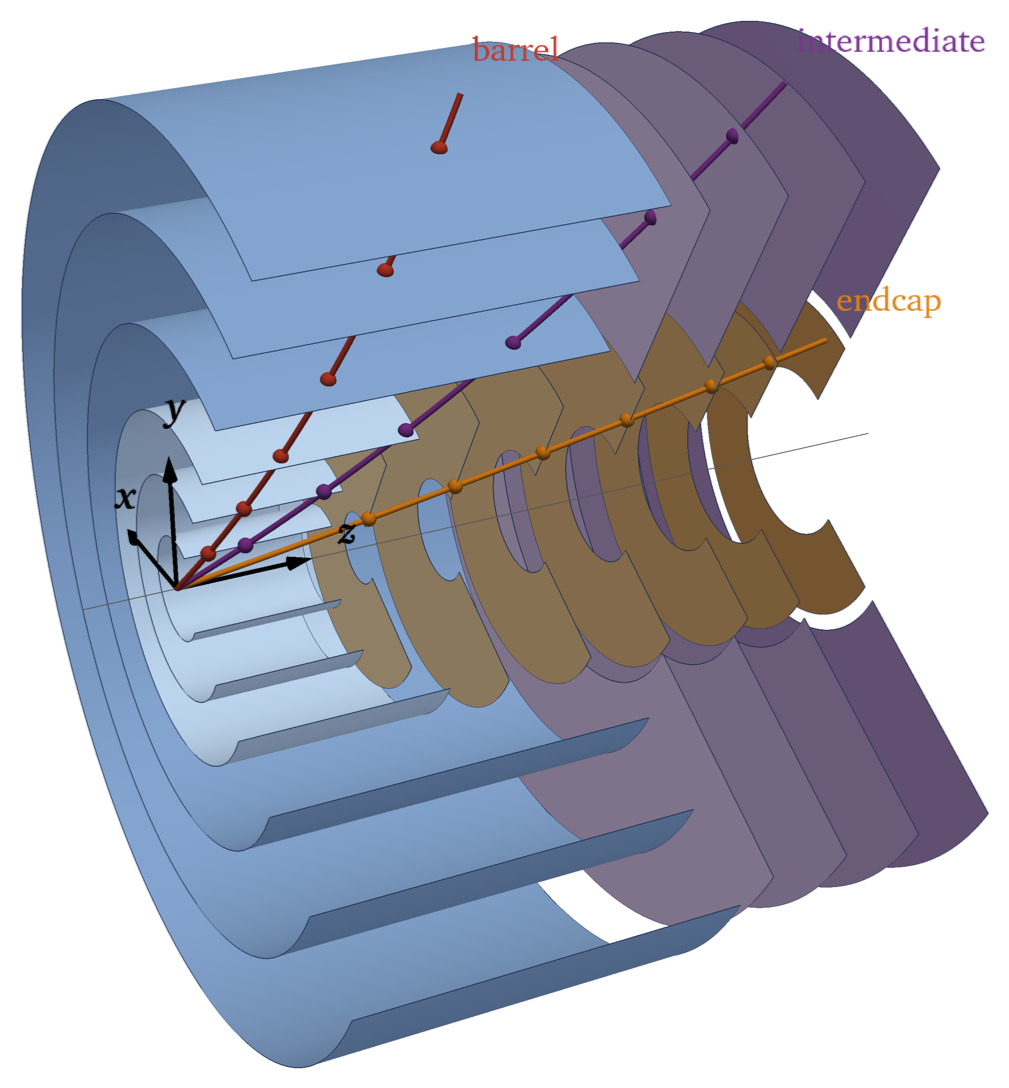
\includegraphics[width=0.85\textwidth]{fig_detector_3d_a.png}
  \caption{The inner and outer trackers of the MUSIC detector, for $z\ge0$, with the quarter facing
  the viewer cut away: barrel layers in blue (IT light, OT dark), IT disks in tan and OT disks in
  lavender. Three tracks from the interaction point, with their hits, illustrate the three regions
  of section~\ref{sec:fakes}: barrel ($\vartheta=65^\circ$), intermediate ($40^\circ$) and endcap
  ($15^\circ$). They are drawn with $\pT=4$~GeV/$c$ so that the bending in the 5~T field is
  visible.}
  \label{fig:det3d}
\end{figure}

\begin{figure}[htbp]
  \centering
  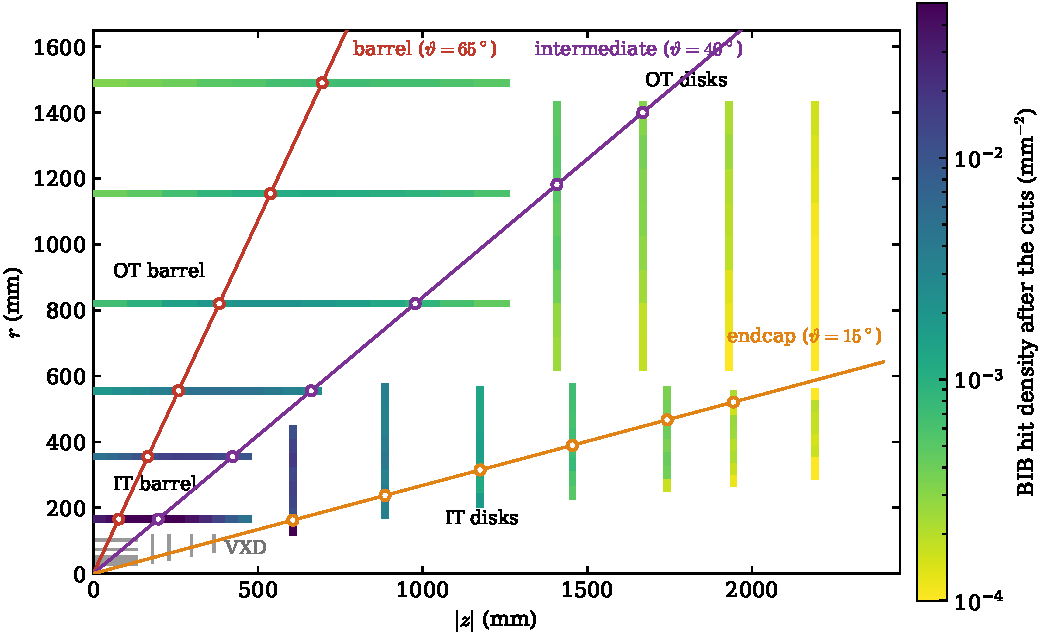
\includegraphics[width=\textwidth]{fig_detector_rz}
  \caption{Quarter view of the inner and outer trackers in $(|z|,r)$, to scale: the six barrel layers
  and the eleven disks of each endcap, coloured by the BIB hit density after the selection of
  section~\ref{sec:selection} (as a function of $|z|$ on the barrel layers and of $r$ on the disks,
  both ends together); the vertex detector, not used here, in grey. The three straight tracks from
  the interaction point, with their hits, are examples of the three regions of
  section~\ref{sec:fakes}.}
  \label{fig:rz}
\end{figure}

\paragraph{Background sample.} One bunch crossing of BIB, the sum of the samples of the
$\mu^+$ and $\mu^-$ beams and of the incoherent pair production at the interaction point,
\todo{provenance: generation with FLUKA, detector simulation; who produced it and which version},
gives 17.3 million hits in the tracker, of which 10.4 million are in the IT and OT (7.7 million in
the six barrel layers). Each hit
has its position, its local sensor coordinates, its time and the momentum of the particle that
produced it, from which its direction is computed.

\paragraph{Signal sample.} 100\,000 single muons, with transverse momenta from 1.5~GeV/$c$
upwards, polar angles between $10^\circ$ and $170^\circ$, full azimuth and a longitudinal vertex
spread of 1.5~mm. Only the hits of the muon itself are used; those of secondary particles (delta
rays) are left out. For the efficiency for high-momentum tracks we extrapolate to
$\pT\to\infty$ (appendix~\ref{app:eff}).

\paragraph{Resolutions.} The simulated hits are exact. We add Gaussian smearing to represent the
detector: $\sigma=100~\mu$m on both local coordinates, $\sigma_t=100$~ps on the time and
$\sigma_\alpha=1.5^\circ$ on each of the two angles that define the hit direction relative to the
sensor. The same smearing is applied to signal and background. The position and time values are
conventional for present-day pixel detectors with timing; a per-hit direction measurement of
$1.5^\circ$ does not exist today in a single sensor and is used here as a working hypothesis, whose
consequences section~\ref{sec:scans} quantifies.

\begin{table}[htbp]
  \centering
  \caption{The barrel layers and the endcap disks of the IT and OT: position, extent, sensitive area
  (for the disks, of both endcaps together), and the mean BIB hit density before and after the
  selection of section~\ref{sec:selection}.}
  \label{tab:layers}
  \small
  \begin{tabular}{lrrrrrr}
    \toprule
    layer & position (mm) & extent (mm) & area (m$^2$) & \multicolumn{2}{c}{density (mm$^{-2}$)} & rejection \\
          &               &             &              & before & after & \\
    \midrule
    IT barrel L0 & $R=165$  & $|z|<482$  & 1.04 & 1.58   & $3.9\times10^{-2}$ & 40 \\
    IT barrel L1 & $R=355$  & $|z|<482$  & 2.20 & 0.552  & $1.1\times10^{-2}$ & 49 \\
    IT barrel L2 & $R=555$  & $|z|<692$  & 5.17 & 0.244  & $3.7\times10^{-3}$ & 66 \\
    OT barrel L0 & $R=820$  & $|z|<1264$ & 14.0 & 0.101  & $1.3\times10^{-3}$ & 77 \\
    OT barrel L1 & $R=1154$ & $|z|<1264$ & 19.5 & 0.0603 & $8.4\times10^{-4}$ & 72 \\
    OT barrel L2 & $R=1491$ & $|z|<1264$ & 28.6 & 0.0356 & $5.4\times10^{-4}$ & 66 \\
    \midrule
    IT disk D0 & $|z|=606$  & $116<r<451$ & 1.33 & 0.273  & $1.7\times10^{-2}$ & 16 \\
    IT disk D1 & $|z|=886$  & $166<r<578$ & 2.12 & 0.153  & $3.6\times10^{-3}$ & 43 \\
    IT disk D2 & $|z|=1175$ & $201<r<567$ & 2.02 & 0.106  & $1.4\times10^{-3}$ & 77 \\
    IT disk D3 & $|z|=1455$ & $225<r<576$ & 1.98 & 0.0774 & $6.5\times10^{-4}$ & 119 \\
    IT disk D4 & $|z|=1743$ & $249<r<570$ & 1.86 & 0.0588 & $3.7\times10^{-4}$ & 161 \\
    IT disk D5 & $|z|=1944$ & $266<r<557$ & 1.72 & 0.0486 & $2.0\times10^{-4}$ & 239 \\
    IT disk D6 & $|z|=2192$ & $287<r<563$ & 1.66 & 0.0425 & $1.4\times10^{-4}$ & 303 \\
    OT disk D0 & $|z|=1408$ & $618<r<1435$ & 13.9 & 0.0257 & $4.4\times10^{-4}$ & 59 \\
    OT disk D1 & $|z|=1669$ & $618<r<1435$ & 13.9 & 0.0276 & $2.9\times10^{-4}$ & 96 \\
    OT disk D2 & $|z|=1931$ & $618<r<1435$ & 13.9 & 0.0231 & $1.9\times10^{-4}$ & 123 \\
    OT disk D3 & $|z|=2192$ & $618<r<1435$ & 13.9 & 0.0228 & $1.1\times10^{-4}$ & 202 \\
    \bottomrule
  \end{tabular}
\end{table}

% =====================================================================
\section{Per-hit observables}\label{sec:obs}

A particle from the interaction point reaches each layer at a predictable time and with a direction
that points back to the beam line. Three observables, computed for each hit from its position, time
and direction alone, measure how far the hit is from this hypothesis.

\paragraph{Longitudinal intercept $z_0$.} In the meridian plane containing the beam axis and the
hit, the hit direction defines a straight line through the hit. Its intersection with the beam axis
is
\begin{equation}
  z_0 = z - r\,\frac{p_z}{p_r},
\end{equation}
where $r$ and $z$ are the hit coordinates and $p_r$, $p_z$ the radial and longitudinal components of
the direction. In a solenoidal field the trajectory projected on the meridian plane is a straight
line, so a particle from the interaction point has $z_0$ within the luminous region, smeared by the
direction resolution.

\paragraph{Transverse momentum from the direction.} In the transverse plane, the circle through the
origin and the hit, tangent at the hit to the transverse direction, has curvature
\begin{equation}
  \frac1R = \frac{2\sin\psi}{r},
\end{equation}
where $\psi$ is the angle between the transverse direction and the radial direction. It is the
curvature a particle from the beam line would need to reach the hit in that direction, and gives
the transverse momentum $\pT=0.3\,B\,R$ (GeV/$c$, T, m). The cut is on $|1/R|$, which is finite and
continuous at infinite momentum.

\paragraph{Corrected time $\tc$.} The time of flight of a muon from the interaction point to the hit
along that helix, $s/(\beta c)$, is subtracted from the hit time. The path length $s$ is the arc of
the circle above divided by $\sin\vartheta$, the polar angle taken from the hit direction, and the
speed $\beta$ follows from the momentum estimated from the curvature and the muon mass. For a muon
from the collision $\tc$ is zero within the time resolution; for a background hit it carries the
delay of the background particle.

\paragraph{Distributions.} Figure~\ref{fig:obs} shows the three observables in the four parts of
the IT and OT for background and signal hits, each after the cuts on the other two observables. The signal peaks
sharply: $\tc$ within the time resolution, $z_0$ within a few centimetres in the IT and about a
decimetre in the OT, where the lever arm of the direction measurement is longer, and the curvature
within the range of the muon momenta. The background is broad in all three. Its corrected time
peaks about 0.3--0.5~ns late, with a long tail of delayed hits and a smaller population arriving
early. \todo{the origin of the late peak is not yet understood; Monte Carlo truth may explain it}
In the endcaps the background time distribution is broader, and the $z_0$ of the background is
much closer to that of the signal: on a disk the direction measures the polar angle of a track
crossing at small angle to the beam, with a short lever arm towards the axis, and in the OT endcap
the two $z_0$ distributions nearly coincide.

\begin{figure}[htbp]
  \centering
  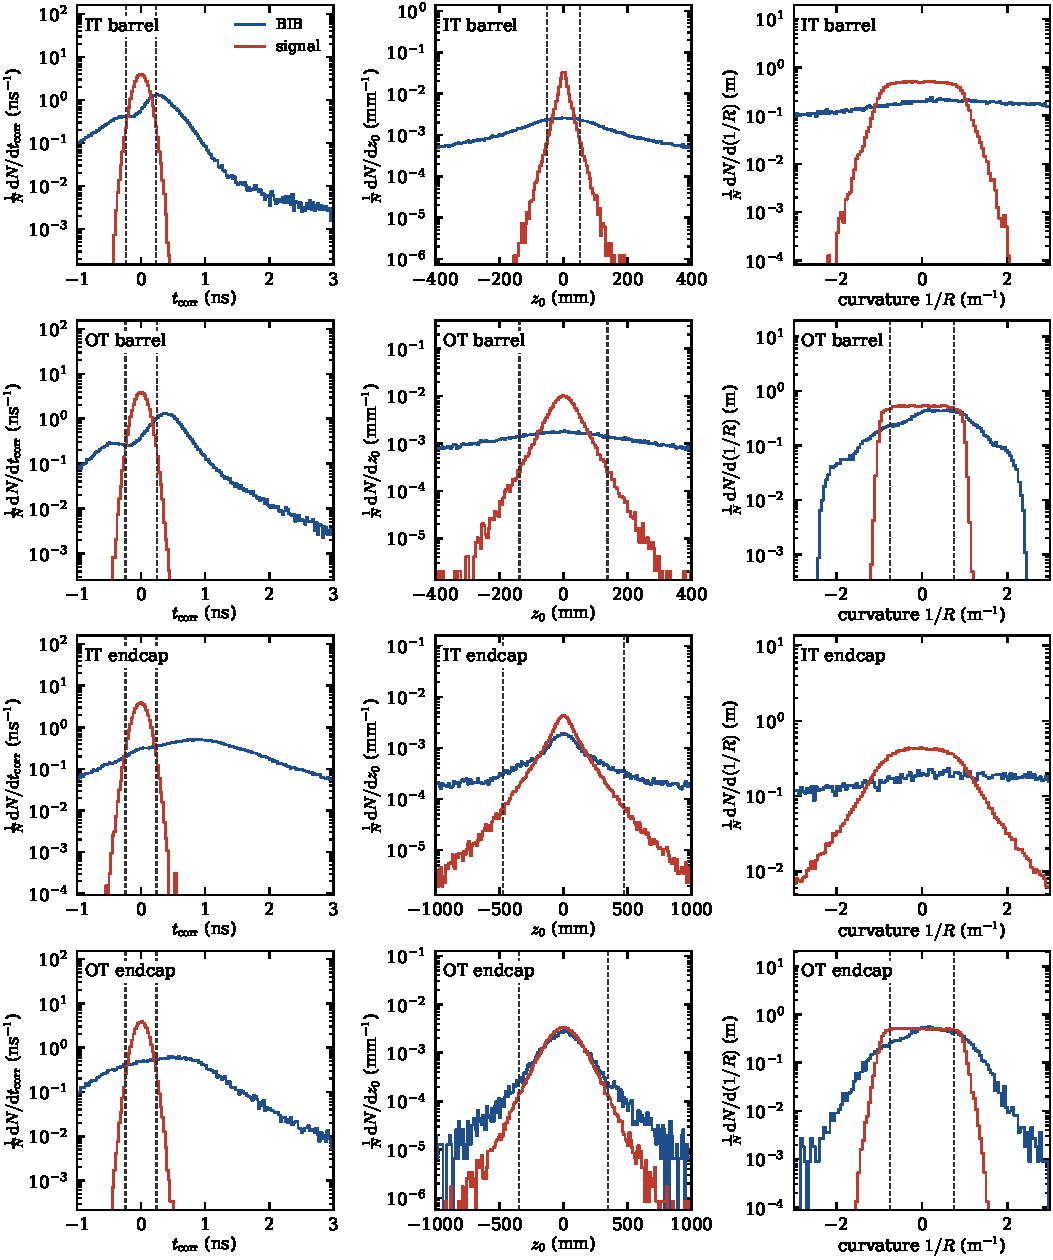
\includegraphics[width=\textwidth]{fig_observables}
  \caption{Corrected time, longitudinal intercept and curvature of the hits in the IT barrel, OT
  barrel, IT endcaps and OT endcaps (top to bottom), for one bunch crossing of background (blue) and for signal muons (red),
  each normalized to unit area. Each distribution is shown after the cuts on the other two
  observables (N$-$1); the dashed lines are the cuts of table~\ref{tab:cuts}. No curvature cut is
  applied in the IT. Note the wider $z_0$ range in the endcaps.}
  \label{fig:obs}
\end{figure}

% =====================================================================
\section{Selection}\label{sec:selection}

\paragraph{Construction of the cuts.} Each subsystem has a symmetric window on $\tc$ and on $z_0$,
and the OT has in addition a minimum transverse momentum of 2~GeV/$c$ (a maximum $|1/R|$). The time
and $z_0$ windows are set to keep 98\% of the signal hits in their N$-$1 distributions, that is
among the hits passing the other cuts. Since each window depends on the other, they are found
together by iteration, which converges in two or three steps. The cuts are thus fixed by the signal
alone, not tuned on the background, and they follow automatically when a resolution changes.
Table~\ref{tab:cuts} lists them.

\begin{table}[htbp]
  \centering
  \caption{Cuts, background rejection factor and signal hit efficiency in the four parts of the IT
  and OT. Rejection factor: hits before over hits after the cuts, for each cut alone and (in
  parentheses) on top of the other two. Efficiency: fraction of the muon's own hits kept,
  extrapolated to $\pT\to\infty$, for each cut alone.}
  \label{tab:cuts}
  \small
  \begin{tabular}{llrrrr}
    \toprule
            &           & IT barrel & OT barrel & IT endcaps & OT endcaps \\
    \midrule
    $|\tc|$ & cut       & 0.233 ns   & 0.245 ns   & 0.242 ns   & 0.241 ns \\
            & rejection & 10.3 (4.6) & 10.2 (5.8) & 16.0 (8.4) & 25.4 (4.9) \\
            & efficiency& 98.4\%     & 98.7\%     & 98.2\%     & 98.4\% \\
    $|z_0|$ & cut       & 52 mm      & 137 mm     & 474 mm     & 349 mm \\
            & rejection & 10.5 (4.7) & 7.8 (3.6)  & 4.5 (2.3)  & 9.0 (1.1) \\
            & efficiency& 98.4\%     & 99.4\%     & 97.8\%     & 98.5\% \\
    $\pT$   & cut       & ---        & 2 GeV/$c$  & ---        & 2 GeV/$c$ \\
            & rejection & ---        & 1.8 (1.8)  & ---        & 3.4 (1.5) \\
            & efficiency& ---        & 100\%      & ---        & 99.9\% \\
    \midrule
    all     & rejection & 48.6       & 72.0       & 37.4       & 96.6 \\
            & efficiency& 96.9\%     & 98.1\%     & 96.1\%     & 96.9\% \\
    \bottomrule
  \end{tabular}
\end{table}

\paragraph{Background rejection.} Together the cuts reduce the background in the IT and OT from
10.4 million to 185\,000 hits per bunch crossing, a factor of 57, with factors between 37 and 97
in the four parts. In the barrel the time and $z_0$ cuts are comparably powerful, a factor of about
ten each alone and four to six on top of the others; the momentum cut adds a factor of two in the
OT. In the endcaps the time cut does most of the work, while the $z_0$ cut adds little on top of the
others, only 1.1 in the OT endcaps. The densities after the cuts range from
$3.9\times10^{-2}$~mm$^{-2}$ in the innermost IT layer to about $10^{-4}$~mm$^{-2}$ on the outermost
disks; the rejection grows with the distance from the interaction point, from 16 on the first IT
disk to 300 on the last (table~\ref{tab:layers}, figure~\ref{fig:density}).

\paragraph{Signal efficiency.} The cuts keep 96--98\% of the hits of high-momentum muons in the
four parts, 96.8\% overall. A track is counted as found if at least five of its hits in the
IT and OT survive (vertex-detector hits are not counted); the track-finding efficiency for
$\pT\to\infty$ is $97.9\pm0.2\%$ (figure~\ref{fig:eff}), and $98.1\pm0.3\%$ for muons confined to
the barrel. It falls below about 2.5~GeV/$c$, where the momentum cut of the OT and the curvature
of the track remove hits.

\begin{figure}[htbp]
  \centering
  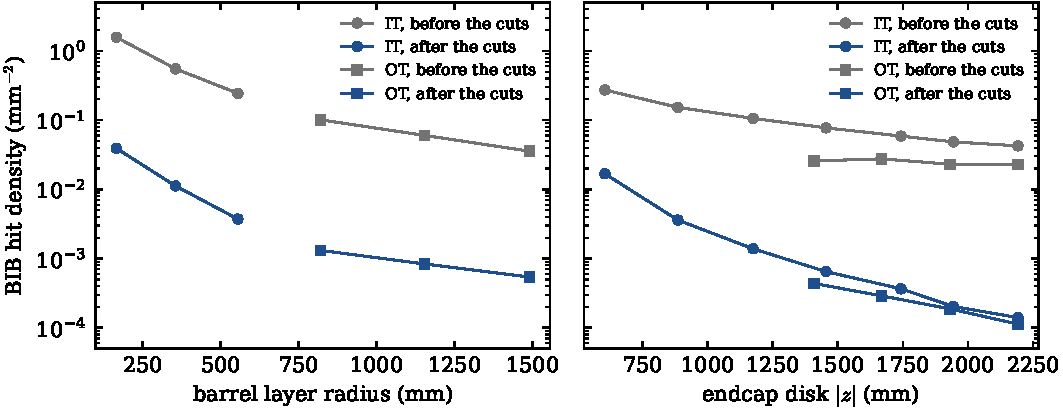
\includegraphics[width=\textwidth]{fig_density}
  \caption{Mean BIB hit density in the barrel layers (left) and endcap disks (right) of the IT
  (circles) and OT (squares), before and after the cuts.}
  \label{fig:density}
\end{figure}

\begin{figure}[htbp]
  \centering
  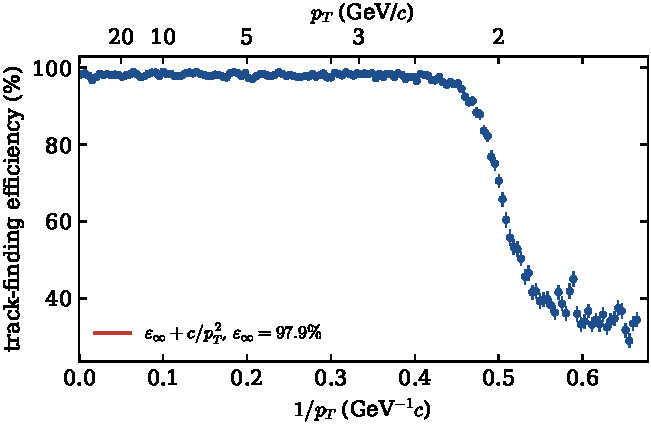
\includegraphics[width=0.6\textwidth]{fig_efficiency}
  \caption{Track-finding efficiency (at least five surviving IT and OT hits) against $1/\pT$,
  with the fit $\varepsilon_\infty+c/\pT^2$ to the muons above 10~GeV/$c$.}
  \label{fig:eff}
\end{figure}

% =====================================================================
\section{Fake tracks after the selection}\label{sec:fakes}

\paragraph{The limit.} Paper~\cite{Paper1} shows that the expected number of combinations of
background hits that pass the goodness-of-fit cut of a track fit, with hits on at least $k$ of the
layers, is a lower limit on the number of fake tracks of any reconstruction algorithm that keeps the
efficiency for real tracks given by that cut. For layers of any shape and noise densities $\rho_i$
that vary across them,
\begin{equation}
  E(\ge k) = \int\mathrm{d}^4\theta \sum_{\substack{S\subseteq C(\theta)\\|S|\ge k}}
  V_{\ndof}\,c_S^{\ndof/2}\sqrt{\det\!\left(J_S^\mathsf{T}J_S\right)}\prod_{i\in S}\rho_i\,\sigma^2 ,
  \label{eq:E}
\end{equation}
where $\theta$ are the helix parameters, $C(\theta)$ the layers crossed, $J_S$ the derivatives of
the crossing points on the layers of $S$ in units of the resolution, $c_S$ the $\chi^2$ cut and
$V_d$ the volume of the unit $d$-sphere. The layers are the six barrel cylinders and the eleven disks
of each endcap, with their actual extents. We require at least five layers, with a one-sided
$3\sigma$ cut for each set of layers. The integral is evaluated by sampling helices with $\pT$
above 10~GeV/$c$ and polar angles in both hemispheres, with the densities after the cuts taken from
the background sample as functions of $|z|$ on each barrel layer and of $r$ on each disk; the
azimuthal symmetry of the BIB lets us sample a narrow range of azimuth.

\paragraph{Three regions.} Each combination is assigned to a region by the layers it uses: the
\emph{barrel} if all its layers are barrel cylinders, the \emph{endcap} if all are disks, and the
\emph{intermediate} region if it uses both. Every combination belongs to exactly one region, and the
three add up to the total. Figure~\ref{fig:towers} illustrates what a combination looks like in each
region: the pieces of the layers crossed by a narrow bundle of tracks, with one track and a few
background hits.

\begin{figure}[htbp]
  \centering
  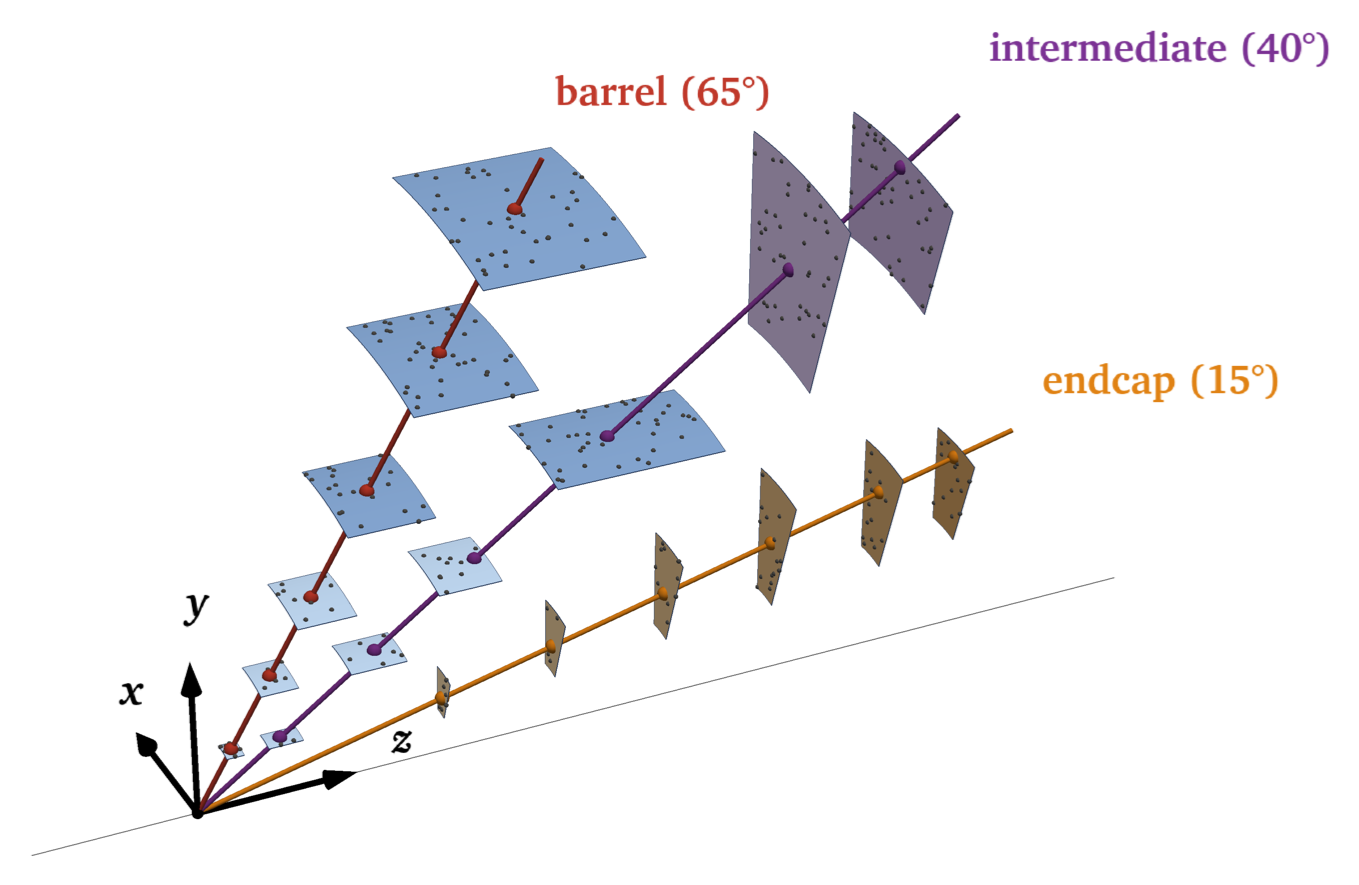
\includegraphics[width=0.9\textwidth]{fig_towers.png}
  \caption{One ``tower'' per region at its true position: the pieces of the actual layers crossed by
  a bundle of tracks from the interaction point within $\pm6^\circ$ in polar angle and $\pm9^\circ$
  in azimuth, around a track (with its hits) at $\vartheta=65^\circ$ (barrel: six barrel layers),
  $40^\circ$ (intermediate: four barrel layers and two OT disks) and $15^\circ$ (endcap: six IT
  disks). Colours as in figure~\ref{fig:det3d}. The small grey spheres are background hits, drawn
  for illustration only: their number is proportional to the area of each piece, not to the actual
  density. The expected numbers of fakes of table~\ref{tab:regions} are for the whole regions, not
  for these towers.}
  \label{fig:towers}
\end{figure}

\paragraph{The acceptance.} The limit refers to a given acceptance: the tracks that the algorithm
must find. Real tracks come from the luminous region, and restricting the longitudinal origin of
the fitted track removes the fakes that point elsewhere at no cost in efficiency. We take a
luminous region of 1.5~mm, the bunch length foreseen at a 10~TeV
collider~\cite{IMCC:2024interim}, and require $|z_0|<4.5$~mm for the fitted track. This
\emph{track} $z_0$ should not be confused with the per-hit $z_0$ of section~\ref{sec:obs}, whose cut
is tens of millimetres wide: the fit of five or six hits measures the origin of a real track to
0.1--0.3~mm. Without it the IT and OT would have 1.4 expected fakes per bunch crossing; with it,
76 times fewer.

\paragraph{Results.} Table~\ref{tab:regions} gives the expected fakes in the three regions. With
$|z_0|<4.5$~mm the IT and OT together have
\begin{equation}
  E(\ge5) = 1.9\times10^{-2}\ \text{fakes per bunch crossing},
\end{equation}
almost entirely from five-layer combinations: the six-layer term is $3\times10^{-6}$. The barrel
contributes 90\%, the intermediate region 9\%, and the endcaps a negligible $10^{-4}$ of the total.
Figure~\ref{fig:polar} shows how the fakes are distributed in polar angle. In the barrel they
concentrate at $45^\circ<\vartheta<76^\circ$ (both hemispheres folded together): the background
density after the cuts is highest at intermediate $|z|$ in every layer, up to 1.4--1.8 times its
mean, and these tracks cross the layers there, obliquely. The intermediate region covers
$30^\circ$--$53^\circ$ and the endcaps $13^\circ$--$34^\circ$. The endcaps are so quiet because
the densities on the disks after the cuts are low, $10^{-4}$--$10^{-3}$~mm$^{-2}$ except on the
first IT disk.

\begin{table}[htbp]
  \centering
  \caption{Expected fakes per bunch crossing in the IT and OT (both endcaps, full azimuth), at least
  five layers, by region, with and without the restriction on the longitudinal origin of the
  fitted track. The statistical uncertainties of the integration are below 1\%.}
  \label{tab:regions}
  \begin{tabular}{lrrl}
    \toprule
    region & $|z_0|<4.5$~mm & no $z_0$ restriction & polar angle (10--90\%) \\
    \midrule
    barrel       & $1.7\times10^{-2}$ & 1.1  & $45^\circ$--$76^\circ$ \\
    intermediate & $1.7\times10^{-3}$ & 0.27 & $30^\circ$--$53^\circ$ \\
    endcap       & $1.5\times10^{-6}$ & $2.7\times10^{-4}$ & $13^\circ$--$34^\circ$ \\
    \midrule
    total        & $1.9\times10^{-2}$ & 1.4 & \\
    \bottomrule
  \end{tabular}
\end{table}

For comparison, one projective tower of six square planes with an outermost plane of 1~m$^2$,
placed at $\vartheta=90^\circ$, gives $4.1\times10^{-3}$: the simplest example of
ref.~\cite{Paper1}, with the measured densities. Since the five-layer terms dominate, the expected
number grows as the fifth power of a common scale factor of the densities; one fake per crossing is
reached at 2.2 times the simulated density (figure~\ref{fig:lambda}). The number of distinct fakes
is smaller than $E$ by the factor $e^{-\eta/2}$, where the window occupancy $\eta$ measures how often
accepted combinations share hits~\cite{Paper1}; we expect $\eta\ll1$ at these densities
\todo{compute $\eta$ for the three regions}.

\begin{figure}[htbp]
  \centering
  \begin{minipage}[t]{0.49\textwidth}\centering
    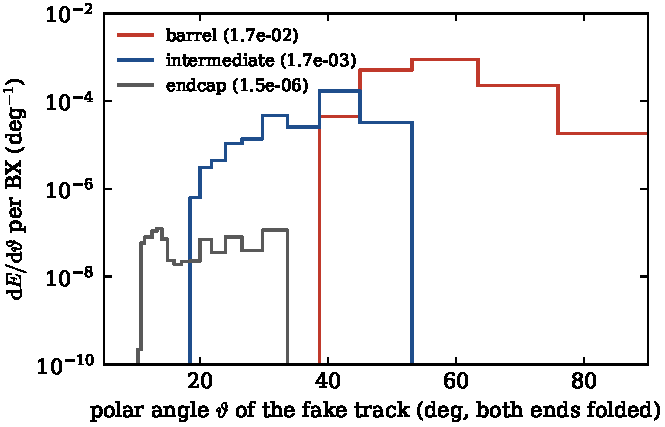
\includegraphics[width=\textwidth]{fig_polar}
    \caption{Distribution of the expected fakes in polar angle, for the three regions, with
    $|z_0|<4.5$~mm (both hemispheres together). The binning follows equal steps in
    $\cot\vartheta$.}
    \label{fig:polar}
  \end{minipage}\hfill
  \begin{minipage}[t]{0.49\textwidth}\centering
    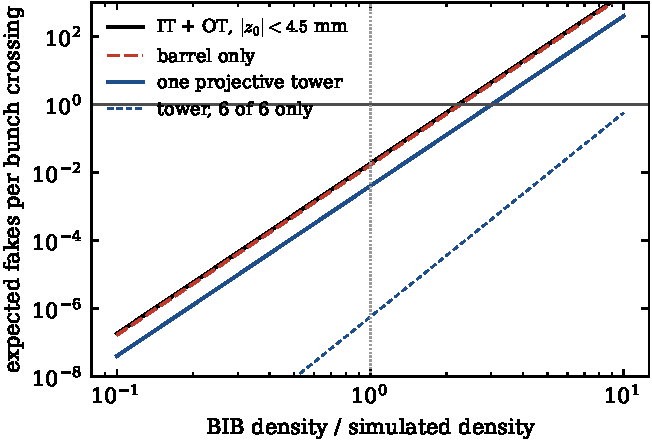
\includegraphics[width=\textwidth]{fig_density_factor}
    \caption{Expected fakes per bunch crossing against a common scale factor of the background
    densities: IT and OT, barrel alone, and one projective tower.}
    \label{fig:lambda}
  \end{minipage}
\end{figure}

\paragraph{Margin.} A factor 2.2 in density is the margin against an underestimate of the BIB in
the simulation, against statistical fluctuations of a single simulated bunch crossing, and against
everything the limit leaves out (section~\ref{sec:discussion}). Equivalently, at the simulated
density the limit stays below one per crossing for resolutions up to about twice the assumed ones
(section~\ref{sec:scans}).

% =====================================================================
\section{Resolution requirements}\label{sec:scans}

\paragraph{Scans.} We vary one resolution at a time around the operating point (100~$\mu$m,
100~ps, $1.5^\circ$), from ten times better to ten times worse, keeping the other two fixed. At
every point the time and $z_0$ cuts are derived again at 98\% signal containment, so the efficiency
stays constant by construction, and the background densities after the cuts and the fake-track
limit are recomputed. The scans are done for the barrel, which contains 90\% of the fakes.
Figure~\ref{fig:scans} shows the limit for one tower and for the whole barrel, scaled from the tower
by their ratio at the operating point (4.1), and the track-finding efficiency. The level of one fake
per crossing in the whole barrel is reached at a position resolution of
200~$\mu$m, a time resolution of 220~ps or a direction resolution of $4.1^\circ$.

\begin{figure}[htbp]
  \centering
  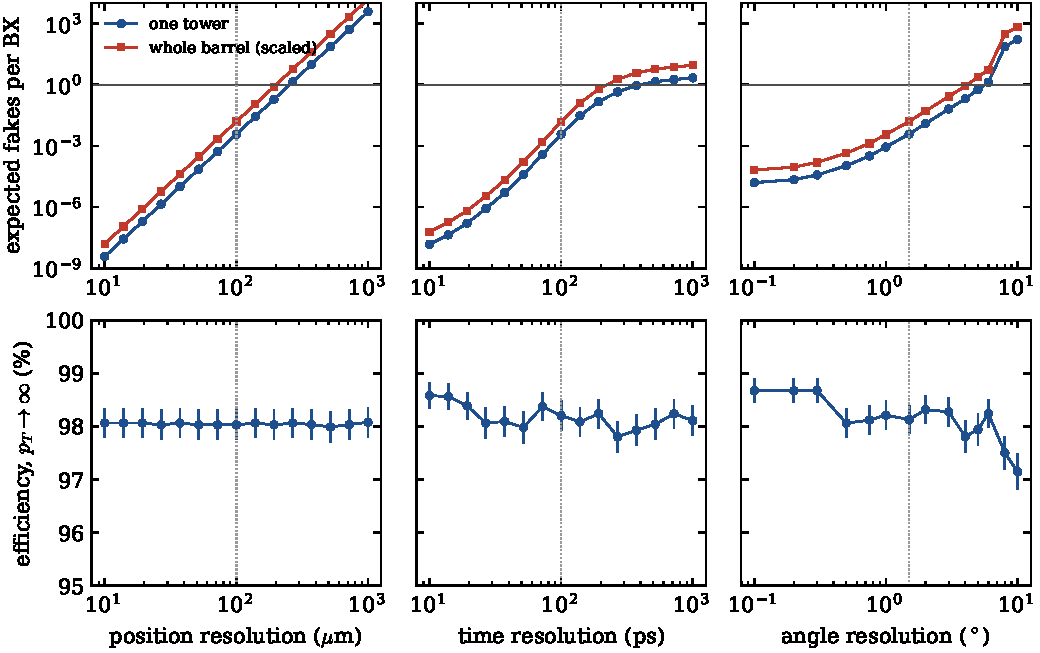
\includegraphics[width=\textwidth]{fig_scans}
  \caption{Top: expected fakes per bunch crossing against the position, time and direction
  resolutions, varied one at a time around the operating point (dotted line), for one projective
  tower (blue) and for the whole barrel with $|z_0|<4.5$~mm (red, scaled from the tower by their
  ratio at the operating point). Bottom: track-finding efficiency for $\pT\to\infty$ of muons
  confined to the barrel.}
  \label{fig:scans}
\end{figure}

\paragraph{Why the curves differ.} The position resolution enters twice: through the per-hit
observables, whose cuts barely change, and through the $\chi^2$ cut of the track fit, which makes
the probability of a five-layer combination scale as $\sigma^6$~\cite{Paper1}. The limit therefore
falls by six orders of magnitude for a ten-fold improvement, steadily over the whole range. The time
and direction resolutions enter only through the cuts, by changing the density of background hits
that survive them, raised to the fifth power. The time scan is steep around the operating point,
where the time window cuts into the late peak of the background; at a few hundred picoseconds the
window contains the whole peak and the curve flattens, the remaining rejection coming from the
other two cuts. Below 30~ps the improvement continues as the window closes on the prompt tail of the
background. The direction scan is gentler at small angles, where the $z_0$ window is no longer set by the
resolution but by the multiple scattering of the signal muons (10~mm in the IT and 83~mm in the OT
at $0.1^\circ$), and steepens above $3^\circ$; above $6^\circ$
the $z_0$ window of the OT becomes so wide that delayed hits of low-momentum muons curling in the
field enter the time-cut distribution, the OT time window opens to several nanoseconds and the limit
jumps by two orders of magnitude.

\paragraph{Targets for R\&D.} Table~\ref{tab:targets} gives the resolution at which the whole
barrel reaches given levels of the limit, each resolution varied alone. Present-day values of
position and time resolution, 100~$\mu$m and 100~ps, leave a margin of about two in background
density; reaching $10^{-4}$ fakes per crossing, a margin of about six, requires about 45~$\mu$m or
50~ps. A direction measurement better than about $1.3^\circ$ is needed for the limit to stay below
$10^{-2}$; it is the least developed of the three capabilities and the one on which the selection
depends most when it is degraded.

\begin{table}[htbp]
  \centering
  \caption{Resolution at which the expected fakes per bunch crossing in the whole barrel
  ($|z_0|<4.5$~mm, at least five of six layers) reach the given level, with the other two
  resolutions at their operating values (100~$\mu$m, 100~ps, $1.5^\circ$).}
  \label{tab:targets}
  \begin{tabular}{lcccc}
    \toprule
    expected fakes per crossing & 1 & $10^{-2}$ & $10^{-3}$ & $10^{-4}$ \\
    \midrule
    position ($\mu$m) & 200 & 93 & 63 & 43 \\
    time (ps)         & 220 & 94 & 67 & 48 \\
    direction (deg)   & 4.1 & 1.3 & 0.67 & 0.21 \\
    \bottomrule
  \end{tabular}
\end{table}

% =====================================================================
\section{Discussion and limitations}\label{sec:discussion}

\paragraph{The background sample.} The results rest on a single simulated bunch crossing. The
densities after the cuts are measured from 15\,000 to 41\,000 hits per layer. Their Poisson
precision is below 1\%, but hits produced by the same background particle are correlated, and the
limit, through its fifth-power dependence, multiplies any relative error on the densities by five.
Independent smearings of the same sample change the tower limit by 8\% (from $4.1\times10^{-3}$ to
$3.8\times10^{-3}$). The $\mu^+$ and $\mu^-$
samples give consistent densities. \todo{bootstrap over BIB primaries for a proper uncertainty}

\paragraph{What the limit does not include.} The limit counts combinations made only of background
hits, with Gaussian resolution and no multiple scattering, for tracks above 10~GeV/$c$ from the
luminous region. Clusters of several hits from one particle, merged hits, sensor inefficiency and
noise, combinations of background with signal hits and correlated background such as low-momentum
particles curling in the field can only add fakes or lose real tracks. A real algorithm will
produce more fakes than the limit; the limit says how many are unavoidable.

\paragraph{Scans of the other regions.} The resolution scans cover the barrel only. The intermediate
region, with a tenth of the fakes, would cross one fake per crossing at somewhat worse resolutions;
in the endcaps the per-hit $z_0$ is weak and the margin rests on the time cut and on the low
densities, so the time resolution matters most there. \todo{scans per region}

\paragraph{Cut optimization.} The cuts are set by signal containment alone. Optimizing them against
the background, or combining the three observables into one likelihood, may gain further, at the
same efficiency.

% =====================================================================
\section{Conclusions}\label{sec:conclusions}

With a time and a direction measured on every hit, three cuts that test the compatibility of each
hit with a particle from the interaction point reduce the beam-induced background in the inner and
outer trackers of a 10~TeV muon collider by a factor of 57, keeping 97\% of the signal hits and
98\% of the tracks. With present-day position and time resolutions, 100~$\mu$m and
100~ps, and a direction resolution of $1.5^\circ$, the algorithm-independent lower limit on fake
tracks is $1.9\times10^{-2}$ per bunch crossing, 90\% of it in the barrel, 9\% in the intermediate
region and almost nothing in the endcaps; this is a factor 2.2 in background density below one fake
per crossing: the background does not make track reconstruction impossible
in principle. The margin grows rapidly with better resolutions, by six orders of magnitude for a
ten-fold improvement in position resolution, and the scans give the resolutions needed for any
chosen margin. The direction measurement is the most demanding of the three requirements and a
natural target for detector R\&D.

\acknowledgments
\todo{Acknowledgements: the producers of the BIB and signal samples; funding (Fermilab: U.S.
Department of Energy, contract No.\ 89243024CSC000002; INFN); and the use of AI tools, as required
by IOP Publishing.}

% =====================================================================
\appendix
\section{Efficiency for $\pT\to\infty$}\label{app:eff}

The hit and track efficiencies are quoted for $\pT\to\infty$, the limit relevant for the
high-momentum tracks to which the fake limit refers. For muons above 10~GeV/$c$ the efficiency is
fitted with $\varepsilon(\pT)=\varepsilon_\infty+c/\pT^2$, the form expected from multiple
scattering and from the $\pT$-dependent curvature, whose effects on the observables scale as
$1/\pT^2$ in the variance. The fit describes the data well (figure~\ref{fig:eff}); for the track
efficiency it gives $\varepsilon_\infty=97.9\pm0.2\%$ and $c=0.60$~GeV$^2$. \todo{from
docs/efficiency\_pt\_infinity.pdf: justification and checks}

\section{Code and data availability}\label{app:code}

The analysis code, the settings files of the runs used and the scripts that make the figures are
available in a public repository~\cite{code}. \todo{The input samples: on request, or a public
location.}

\IfFileExists{JHEP.bst}{\bibliographystyle{JHEP}}{\bibliographystyle{unsrt}}
\bibliography{refs}

\end{document}
